\paragraph{}{
	L'Unité Arithmétique et Logique, abrégé UAL, permet de faire des calculs
	basiques (additions, divisions, décallages de bits, etc.). Elle effectue
	les calcules sur huit bits. L'UAL a trois entrées. La première sur trois bits
	permet de préciser le code l'opérateur à	effectuer. Les deux autres entrées
	sur hiut bits sont les opérantes de l'opération demandée. \newline
	En sortie, sur \textit{ouput} on peut lire le résultat de l'opération. Il
	y a également quatres drapeaux comme détaillés ci-dessous.
}

\begin{itemize}
	\item[CF] pour \textit{Carrie Flag} est le drapeau levé lorsque que l'opération
	génère une retenue.
	\item[ZF] pour \textit{Zero Flag} qui est armé lorsque que le résultat comporte uniquement
	des $0$.
	\item[OF] pour \textit{Over Flow} qui est un drapeau levé lorsque on dépasse
	la capacité des nombres représentés.
	\item[SF] pour \textit{Sign Flag} qui est levé lorsque le résultat a son
	bit de poids fort à $1$, c'est un nombre signé.
\end{itemize}

\begin{figure}
	\centering
	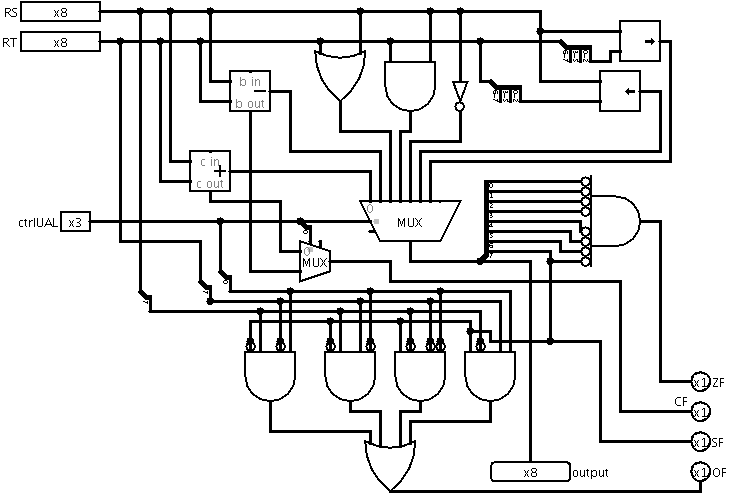
\includegraphics[scale=0.4,origin=c]{circuits/UAL.png}
	\label{ual_circ}
	\caption{Sch\'{e}ma \'{e}lectronique de l'Unit\'{e} Arithm\'{e}tique et Logique}
\end{figure}

\begin{figure}
	\begin{center}
	\begin{tabular}{|c|c|c|c|c|}
		\hline
		\backslashbox{b3b2}{b1b0} & $0$ & $01$ & $11$ & $10$ \\ 
		\hline 
		$00$ & $0$ & $0$ & $0$ & $0$ \\ 
		\hline 
		$01$ & $0$ & $0$ & $0$ & $0$ \\ 
		\hline 
		$11$ & $1$ & $1$ & $0$ & $1$ \\ 
		\hline 
		$10$ & $1$ & $1$ & $1$ & $1$ \\ 
		\hline 
	\end{tabular} 
	\end{center}
	\label{karnaugh_ual}
	\caption{Tableau de Karnaugh pour le décodage de \textit{ctrlUAL}}
\end{figure}

\paragraph{}{
	Le schéma électronique de l'UAL est présenté à la figure \ref{ual_circ}.
	La partie qui décode le signal \textit{ctrlUAL} correspond au tableau de
	Karnaugh de la figure \ref{karnaugh_ual} duquel on extrait l'équation :
	\begin{equation}
		b3 . \neg(b2) + b3 . b2 \neg(b1) + b3 . b1 \neg(b0)
		\label{equation_ual}
	\end{equation}
	Cette équation nous permet alors de réaliser le circuit électronique 
	décodant \textit{ctrlAUL}.
}